\documentclass[12pt,letterpaper]{article}
\usepackage{graphicx,textcomp}
\usepackage{natbib}
\usepackage{setspace}
\usepackage{fullpage}
\usepackage{color}
\usepackage[reqno]{amsmath}
\usepackage{amsthm}
\usepackage{fancyvrb}
\usepackage{amssymb,enumerate}
\usepackage[all]{xy}
\usepackage{endnotes}
\usepackage{lscape}
\newtheorem{com}{Comment}
\usepackage{float}
\usepackage{hyperref}
\newtheorem{lem} {Lemma}
\newtheorem{prop}{Proposition}
\newtheorem{thm}{Theorem}
\newtheorem{defn}{Definition}
\newtheorem{cor}{Corollary}
\newtheorem{obs}{Observation}
\usepackage[compact]{titlesec}
\usepackage{dcolumn}
\usepackage{tikz}
\usetikzlibrary{arrows}
\usepackage{multirow}
\usepackage{xcolor}
\newcolumntype{.}{D{.}{.}{-1}}
\newcolumntype{d}[1]{D{.}{.}{#1}}
\definecolor{light-gray}{gray}{0.65}
\usepackage{url}
\usepackage{listings}
\usepackage{color}

\definecolor{codegreen}{rgb}{0,0.6,0}
\definecolor{codegray}{rgb}{0.5,0.5,0.5}
\definecolor{codepurple}{rgb}{0.58,0,0.82}
\definecolor{backcolour}{rgb}{0.95,0.95,0.92}

\lstdefinestyle{mystyle}{
	backgroundcolor=\color{backcolour},   
	commentstyle=\color{codegreen},
	keywordstyle=\color{magenta},
	numberstyle=\tiny\color{codegray},
	stringstyle=\color{codepurple},
	basicstyle=\footnotesize,
	breakatwhitespace=false,         
	breaklines=true,                 
	captionpos=b,                    
	keepspaces=true,                 
	numbers=left,                    
	numbersep=5pt,                  
	showspaces=false,                
	showstringspaces=false,
	showtabs=false,                  
	tabsize=2
}
\lstset{style=mystyle}
\newcommand{\Sref}[1]{Section~\ref{#1}}
\newtheorem{hyp}{Hypothesis}

\title{Problem Set 1}
\date{Due: October 8, 2026}
\author{Applied Stats/Quant Methods 1}

\begin{document}
	\maketitle
	
	\section*{Instructions}
	\begin{itemize}
	\item Please show your work! You may lose points by simply writing in the answer. If the problem requires you to execute commands in \texttt{R}, please include the code you used to get your answers. Please also include the \texttt{.R} file that contains your code. If you are not sure if work needs to be shown for a particular problem, please ask.
\item Your homework should be submitted electronically on GitHub.
\item This problem set is due before 23:59 on Thursday October 8, 2026. No late assignments will be accepted.
	\end{itemize}
	
	\vspace{1cm}
	\section*{Question 1: Education}

A school counselor was curious about the average of IQ of the students in her school and took a random sample of 25 students' IQ scores. The following is the data set:\\
\vspace{.5cm}

\lstinputlisting[language=R, firstline=42, lastline=42]{PS01_answers_AS.R}  


\vspace{1cm}

\begin{enumerate}
	\item {\textit{Find a 90\% confidence interval for the average student IQ in the school (As a hint, you first need the mean and SD to create a CI):}}\\
	
	The mean of data set y\\
	\vspace{1cm}
	\lstinputlisting[	language=R, firstline=51, lastline=52]{PS01_answers_AS.R}
	
	\[
	\begin{aligned}
		\bar{y} &= \frac{\sum y_i}{n} \\
		\bar{y} &= \frac{2461}{25} \\
		\bar{y} &= 98.44
	\end{aligned}
	\]
	The standard deviation of the data set y\\
	\vspace{1cm}
	\	\lstinputlisting[	language=R, firstline=53, lastline=54]{PS01_answers_AS.R}
	\[
	\begin{aligned}
	s = \sqrt{\frac{\sum_{i=1}^{n}(y_i-\bar{y})^2}{n-1}}\\
	s = \sqrt{\frac{\sum_{i=1}^{25}(y_i-\bar{y})^2}{25-1}}\\
	s = \sqrt{\frac{4114.16}{24}}\\
	s = \sqrt{171.4233}\\
	s = 13.09
	\end{aligned}
	\]
	
	Find the degrees of freedom
	\[
	\begin{aligned}
	n=25\\
	df=n-1\\
	df=25-1\\
	df=24
	\end{aligned}
	\]	


	Because n $<$ 30, calculate t value\\
	
	For a 90\% confidence interval, the significance level ($\alpha$) is
	
	\[
	\begin{aligned}
	\alpha = 1-0.90 \\
	\alpha = 0.10
	\end{aligned}
	\]
	
	Since the confidence interval is two-sided, divide $\alpha$ by two
	
	\[
	\frac{\alpha}{2} = \frac{0.10}{2}=0.05
	\]
	
	Therefore, 0.95 is used to calculate the t-distribution
	with 24 degrees of freedom.
	

	\vspace{1cm}
	\lstinputlisting[	language=R, firstline=62, lastline=63]{PS01_answers_AS.R}

	\[
	\begin{aligned}
	t^* = 1.711
	\end{aligned}
	\]
	
	
	Using the mean, t statistic, the standard deviation, and the sample size, calculate the confidence interval

	\[
	CI
	=
	\left(
	\bar{x} - t^*\frac{s}{\sqrt{n}},
	\bar{x} + t^*\frac{s}{\sqrt{n}}
	\right)
	\]
	
	\[
	lower bound=98.44-1.711 (\frac{13.09}{\sqrt{25}}).
	\]
	\[
	upper bound=98.44+1.711 (\frac{13.09}{\sqrt{25}}).
	\]
		
	\[
	CI=
	(\text{93.95993},\text{102.9201}).
	\]
	\lstinputlisting[	language=R, firstline=66, lastline=70]{PS01_answers_AS.R}

	
	Therefore, it can be asserted with 90\% confidence that the average student IQ in the school is between 93.95993 and
	102.9201.
	
	
	\item \textit{Next, the school counselor was curious  whether  the average student IQ in her school is higher than the average IQ score (100) among all the schools in the country.}\\ 
	
	
	
	\noindent \textit{Using the same sample, conduct the appropriate hypothesis test with $\alpha=0.05$.}
	
	\paragraph{Assumptions -}
	The IQ data is quantitative, continuous, and interval. The counselor used random sampling to gather the data. The counselor used a  sample size of 25. Since sample size is less than 30, it can be assumed that the population distribution is approximately normal and therefore a t-test can be used. 
	\\
	\paragraph{Hypothesis -}\mbox{}
\begin{list}{}{\setlength{\leftmargin}{2em}\setlength{\rightmargin}{0pt}}
	\item {Null hypothesis: Students' average IQ is equal to 100}
	\[
	H_0: \mu = 100
	\]
	\item {Alternative hypothesis: Students' average IQ is greater than 100}
	\[
	H_1: \mu > 100
	\]
\end{list}

	\noindent{Because the problem is asking only about whether the student's IQ, it is appropriate a one sided right tailed hypothesis test.}
	\paragraph{Test statistic} - Calculate the test statistic using the sample mean, the null hypothesis mean, the standard deviation, and the sample size. The test statistic (measured in units of standard error) measures how far the sample result is from the hypothesized mean.
	\[
	t = \frac{\bar{x} - \mu_0}{s/\sqrt{n}}
	\]	
	\[
	t = \frac{\bar{x} - 100}{13.09287/\sqrt{25}}
	\]
	\[
	t = -0.5957
	\]
	
	\lstinputlisting[	language=R, firstline=83, lastline=84]{PS01_answers_AS.R}
	
	\paragraph{Calculate P-value} - Calculate the p-value using the test statistic and the t-distribution with 24 degrees of freedom.P value is the probability of observing the test statistic. In this case, using a right-tailed test, the p- value calculates the probability of a value greater than 100 occurring. 
	\[
	p = P(T_{df} \geq t)
	\]
	\[
	p=P(T_{24}\geq -0.5957)=0.721
	\]
	\[
	p = 0.721 > \alpha = 0.05
	\]
	\lstinputlisting[	language=R, firstline=88, lastline=89]{PS01_answers_AS.R}
	
	\paragraph{conclusion} - Because the p value is 0.7125 whitch is greater than the significance level of .05 we fail to reject the null hypothesis that the students' average IQ is equal to 100. Therefore, there is insufficient evidence to conclude that the students' IQ average IQ is greater than 100.   

\end{enumerate}

\newpage

	\section*{Question 2: Political Economy}

\noindent Researchers are curious about what affects the amount of money communities spend on addressing homelessness. The following variables constitute our data set about social welfare expenditures in the USA. \\
\vspace{.5cm}


\begin{tabular}{r|l}
	\texttt{State} &\emph{50 states in US} \\
	\texttt{Y} & \emph{per capita expenditure on shelters/housing assistance in state}\\
	\texttt{X1} &\emph{per capita personal income in state} \\
	\texttt{X2} &  \emph{Number of residents per 100,000 that are "financially insecure" in state}\\
	\texttt{X3} &  \emph{Number of people per thousand residing in urban areas in state} \\
	\texttt{Region} &  \emph{1=Northeast, 2= North Central, 3= South, 4=West} \\
\end{tabular}

\vspace{.5cm}
\noindent Explore the \texttt{expenditure} data set and import data into \texttt{R}.
\vspace{.5cm}
\lstinputlisting[language=R, firstline=103, lastline=103]{PS01_answers_AS.R}  
\vspace{.5cm}
\begin{itemize}

\item
\textit{Please plot the relationships among \emph{Y}, \emph{X1}, \emph{X2}, and \emph{X3}? What are the correlations among them (you just need to describe the graph and the relationships among them)?}
\vspace{.5cm}
 \begin{figure}[H]
 	\centering
 	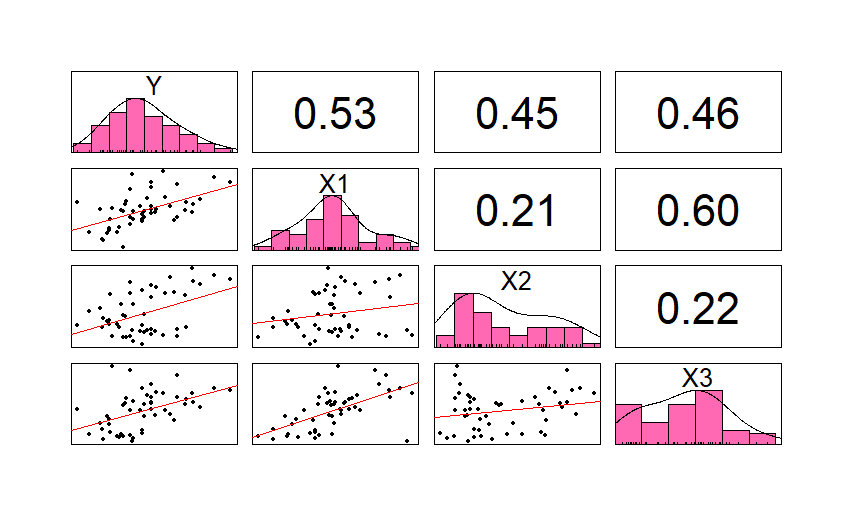
\includegraphics[width=0.8\textwidth]{ps01_q2_p1.png}
 	\caption{Correlations Between Expenditure (Y), Income (X1), Insecure Residents (X2), and Urban Populations (X3)}
 	\label{ps01_q2_p1.png}
 \end{figure}
 
\begin{list}{--}{\setlength{\leftmargin}{2em}}
	\item{Expenditure and Income have a correlation coefficient of .53 which indicates a moderate positive correlation}
	\item{Expenditure and Insecure Residents have a correlation coefficient of .45 which indicates a moderate positive correlation}
	\item{ Expenditure and Urban Population have a correlation coefficient of .46 which indicates a moderate positive correlation}
	\item{Income and Insecure Residents have a correlation coefficient CC of .21 which indicates a weak positive correlation}
	\item{Income and Urban Population have a correlation coefficient CC of .60 which indicates a moderate positive correlation}
	\item{Insecure Residents and Urban Population have a correlation coefficient of .22 which indicates a weak positive correlation}
\end{list}

\item
\textit{Please plot the relationship between \emph{Y} and \emph{Region}? On average, which region has the highest per capita expenditure on housing assistance?}
\vspace{.5cm}

 \begin{figure}[H]
	\centering
	\includegraphics[width=0.8\textwidth]{ps01_q2_p8.png}
	\caption{Expenditure by Region}
	\label{ps01_q2_p8.png}
\end{figure}

On average the western region, has the highest per capita expenditure on housing assistance. The box plot definitively shows that the west has the highest median expenditure. I used the R function below to confirm that the west had the highest mean expenditure with 88.30769, the south's was 69.18750,  the north central's was 79.44444 and the northeast's was 83.91667.  
 
\lstinputlisting[	language=R, firstline=149, lastline=150]{PS01_answers_AS.R}

\item
\textit{Please plot the relationship between \emph{Y} and \emph{X1}? Describe this graph and the relationship. }


 \begin{figure}[H]
	\centering
	\includegraphics[width=0.8\textwidth]{ps01_q2_p9.png}
	\caption{Expenditure vs Income}
	\label{ps01_q2_p9.png}
\end{figure}

The graph above shows a moderate positive coorelation between expenditure and income 

\textit{Reproduce the above graph including one more variable \emph{Region} and display different regions with different types of symbols and colors.}
\end{itemize}
\begin{figure}[H]
	\centering
	\includegraphics[width=0.8\textwidth]{ps01_q2_p10.png}
	\caption{Expenditure vs Income by Region}
	\label{fig:ps01_q2_p10}
\end{figure}
\subsection*{Sources}
\begin{itemize}
	\item \url{https://stat.ethz.ch/R-manual/R-devel/library/lattice/html/splom.html}
	\item \url{https://smin95.github.io/dataviz/basics-of-ggplot2-and-correlation-plot.html}
	\item \url{https://www.overleaf.com/learn/latex/Learn_LaTeX_in_30_minutes}
\end{itemize}
\end{document}
